\chapter{ContainerClasses}

容器

\splitLine

引言

Qt 提供了一系列基于模板的通用容器类,可以用于存储指定类型的元素。例如,如果你需要一个可动态调整大小的 QString 数组,那么你可以使用 QVector<QString>。

这些类的设计目标是比 STL 容器更轻量,更安全,更易用。如果你不熟悉 STL,或想更有“ Qt 范”,使用这些类代替 STL 会是更好的选择。

这些类都是隐式共享和可重入的,并且针对几个方面做了优化,一是速度,二是较低的内存占用,三是尽可能少的内联代码,减少生成程序的体积。另外,在所有线程都以只读的方式访问容器时,这些类是线程安全的。

要遍历容器中的元素,你可以使用两种风格迭代器:Java 风格迭代器和 STL 风格迭代器。Java 风格迭代器有更好的易用性和更高级的函数,而 STL 风格迭代器则在效率上会略有优势,并且可以用于 Qt 和 STL 提供的泛型算法中。

Qt 还提供了 foreach 关键字,可以方便地遍历容器。

注:从 Qt 5.14 开始,绝大部分容器类已经支持范围构造函数,但需要注意的
是 QMultiMap 是一个例外。我们推荐使用该特性代替各种 from/to 方法。例如:

\begin{quote}
译者注:这里的 from/to 方法指的是 Qt 容器类提供的以 from/to 开头的转换方法,如QVector::toList
\end{quote}

\begin{lstlisting}[language=C++]
QVector<int> vector{1, 2, 3, 4, 4, 5};
QSet<int> set(vector.begin(), vector.end());
/*
    将会生成一个 QSet,包含元素 1, 2, 4, 5。
*/
\end{lstlisting}

容器类

\splitLine

Qt 提供了以下几种顺序容器:QList,QLinkedList,QVector,QStack 和 QQueue。对于大多数的应用,QList 是最适用的。虽然其基于数组实现,但支持在头部和尾部快速插入。如果确实需要一个基于链表的列表,你可以使用 QLinkedList;如果要求元素以连续内存的形式保存,那么可以使用 QVector。QStack 和 QQueue提供了 LIFO 和 FIFO 语义的支持。

Qt也提供了一系列关联容器:QMap,QMultiMap,QHash,QMultiHash 和 QSet。"Multi" 容器可以方便地支持键值一对多的情形。“Hash” 容器提供了快速查找的能力,这是通过使用哈希函数代替对有序集合进行二分查找实现的。

较为特殊的是 QCache 和 QContiguousCache,这两个类提供了在有限的缓存中
快速查找元素的能力。


\begin{tabular}{|l|l|}
\hline
类&综述 \\
\hline
QList&	这是目前使用最普遍的容器类,其保存了一个元素类型为T的列表,支持通过索引访问。QList 内部通过数组实现,以确保基于索引的访问足够快。
元素可以通过 QList::append() 和 QList::prepend() 插入到首尾,也可以通过 QList::insert() 插入到列表中间,和其他容器类不同的是,QList 为生成尽可能少的代码做了高度优化。QStringList 继承于 QList<QString>。
QLinkedList)	这个类和 QList 很像,不同的是这个类使用迭代器进行而不是整形索引对元素进行访问。和 QList 相比,其在中间插入大型列表时其性能更优,而且其具有更好的迭代器语义。(在 QLinkedList 中,指向一个元素的迭代器只要该元素存在,则会一直保持有效,而在 QList 的迭代器则可能会在任意的元素插入或删除后失效。)
QVector	这个类以数组的形式保存给定类型的元素,在内存中元素彼此相邻。在
       一个 vector 的头部或中部插入可能会相当慢,因为这可能会导致大量
       元素需要在内存中移动一个位置。\\
\hline
QVarLengthArray<T, Prealloc>&	这个类提供了一个底层的变长数组,在速度极其重要的情况下可以用来代替 QVector\\
QStack&	这个类继承于 QVector,用于为”后进,先出”(LIFO )提供便捷的语
        义支持。其为 QVector 添加了以下方法:QVector::push(),pop() 和
        top()\\
\hline
QQueue&	这个类继承于 QVector,用于为”先进,先出”(FIFO )提供便捷的语
        义支持。其为 QVector 添加了以下方法:QList::enqueue(),
        dequeue() 和 head()\\
\hline
QSet&	这个类提供了一个单值数学集合,支持快速查找\\
\hline
QMap<Key, T>&	这个类提供了一个将类型为Key的键映射到类型为T的值的字典(关联数组)。通常情况下键值是一一对应的。QMap 根据Key进行排序,如果排序无关紧要,使用 QHash 代替速度会更快\\
\hline
QMultiMap<Key, T>&	这个类继承于 QMap,其为诸如键值一对多的多值映射提供了一个友好的接口\\
\hline
QHash<Key, T>&	这个类几乎与 QMap 有完全一致的 API ,但查找效率会有明
               显的提高。QHash 的数据是无序的。\\
\hline
QMultiHash&	这个类继承于 QMap,其为多值映射提供了一个友好的接口\\
\hline
\end{tabular}

容器可以嵌套。例如在键为 QString,值为 QList 时,完全可以使用 QMap<QString, QList>。

容器类的定义位于和容器同名的独立头文件中(例如,<QLinkedList>)。为了方便,在 <QtContainerFwd> 中对所有容器类进行了前置声明。

保存在各个容器中的值类型可以是任意可复制数据类型。为了满足这一要求,该类型必须提供一个复制构造函数和一个赋值运算符。某些操作可能还要求类型支持默认构造函数。对于大多数你想要在容器中保存的类型都满足这些要求,包括基本类型,如 int, double,指针类型,以及 Qt 数据类型,如 QString,QDate 和 QTime,但并不包括 QObject 及其子类(QWidget,QDialog,QTimer 等)。如果你尝试实例化一个 QList<QWidget>,编译器将会抱怨道 QWidget 的复制构造函数和赋值运算符被禁用了。如果需要在容器中保存这些类型的元素,可以保存其指针,如 QList<QWidget *>。

下面是一个满足可赋值数据类型要求的自定义数据类型的例子:

\begin{lstlisting}[language=C++]
class Employee
{
public:
    Employee() {}
    Employee(const Employee &other);

    Employee &operator=(const Employee &other);

private:
    QString myName;
    QDate myDateOfBirth;
};
\end{lstlisting}

如果我们没有提供一个复制构造函数或一个赋值运算符,C++ 将会提供一个表现
为逐个复制成员的默认实现。在上面的例子中,默认行为就足够了。同样的,如
果没有提供默认构造函数,C++ 会提供一个默认构造函数,对成员进行默认构造。
尽管没有提供任何的构造函数或赋值运算符,下面的数据类型可以被保存于容器
中。

\begin{lstlisting}[language=C++]
struct Movie
{
    int id;
    QString title;
    QDate releaseDate;
};
\end{lstlisting}

一些容器对它们所能保存的数据类型有额外的要求。举个例子,QMap<Key, T> 的键类型 Key 必须提供 operator<() 方法。这些特殊要求在类的详细描述中有说明。在某些情况下,特定函数会有特定的要求,这在函数的描述中有说明。如果条件不满足,编译器将总是会报错。

Qt容器提供了 operator<<() 和 operator>>(),因此这些类可以很方便地通过
QDataStream 进行读写。这意味着存储在容器中的元素类型也必须支持
operator<<() 和 operator>>()。支持这一点是很简单的;以下是我们使上面的
Movie 结构体支持这一点所做的改动:

\begin{lstlisting}[language=C++]
QDataStream &operator<<(QDataStream &out, const Movie &movie)
{
    out << (quint32)movie.id << movie.title
        << movie.releaseDate;
    return out;
}

QDataStream &operator>>(QDataStream &in, Movie &movie)
{
    quint32 id;
    QDate date;

    in >> id >> movie.title >> date;
    movie.id = (int)id;
    movie.releaseDate = date;
    return in;
}
\end{lstlisting}

某些容器类的文档中会提到默认值;举个例子,QVector 会自动使用默认值初始化其元素;QMap::value() 在指定键不存在时会返回一个默认值。对于大部分的值类型,这就是简单地代表通过默认构造函数创建的值(例如对于 QString 即空字符串)。但是对于基本类型,如 int 和 double 和指针类型,C++ 语言并没有规定任何的初始化方式,因此在这些情况下,Qt 容器将会自动将其初始化为0。

\splitLine

迭代器类

迭代器提供了一个统一的方式去访问容器中的元素。Qt 容器类提供了两种风格迭代器:Java 风格迭代器和 STL 风格迭代器。两种迭代器均会在容器中的数据被修改或因调用非 const 成员函数导致数据从隐式共享中分离后失效。

\splitLine

Java 风格迭代器

Java 风格迭代器在 Qt4 中引入,作为标准使用在Qt应用中。和 STL 风格迭代器相比,其易用性更高,代价是性能略低。该风格迭代器 API 以 Java 迭代器类为原型设计。

对于每一个容器类,同时提供了两种数据类型的 Java 风格迭代器:一种支持只
读访问,另一种支持读写访问。

\begin{tabular}{|l|l|l|}
\hline
容器&	只读迭代器	&读写迭代器\\
\hline
QList, QQueue&	QListIterator&	QMutableListIterator\\
\hline
QLinkedList	&QLinkedListIterator&	QMutableLinkedListIterator\\
\hline
QVector, QStack	&QVectorIterator&	QMutableVectorIterator\\
\hline
QSet&	QSetIterator&	QMutableSetIterator\\
\hline
QMap<Key, T>, QMultiMap<Key, T>	&QMapIterator<Key, T>&
                                                       QMutableMapIterator<Key,
                                                       T>\\
\hline
QHash<Key, T>, QMultiHash<Key, T>&	QHashIterator<Key, T>&	QMutableHashIterator<Key, T>\\
\hline
\end{tabular}

在接下来的讨论中,我们将重点关注 QList 和 QMap。QLinkedList,QVector 和 QSet 的迭代器类型和 QList 有完全一样的接口,类似的,QHash 和 QMap 的迭代器类型的接口也是相同的。

和 STL 风格迭代器(下一节介绍)不同,Java 风格迭代器指向的是元素间隙而
不是元素本身。因此,Java 风格迭代器可以指向容器最前(在第一个元素之前),
也可以指向容器最后(在最后一个元素之后),还可以指向两个元素之间。下图
用红色箭头展示了一个四个元素的列表容器合法的迭代器位置。

\begin{figure}[hbt!]  
	\centering
    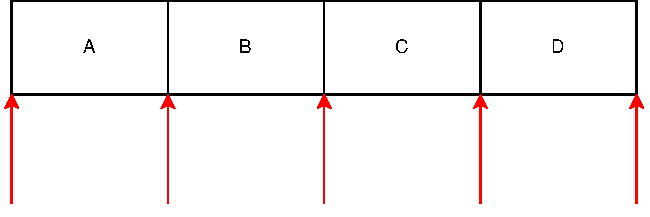
\includegraphics[width=0.5\textwidth]{java_style_iterator.pdf}
	%\caption{model index}
\end{figure}

这是一个通过循环迭代有序遍历 QList<QString> 中的所有元素并打印到终端的
常用写法:

\begin{lstlisting}[language=C++]
QList<QString> list;
list << "A" << "B" << "C" << "D";

QListIterator<QString> i(list);
while (i.hasNext())
    qDebug() << i.next();

\end{lstlisting}

它的工作原理如下:需要被迭代的 QList 对象作为参数传递给 QListIterator 的构造函数。此时迭代器位于列表中第一个元素的前面(位于元素“A“之前)。接着我们调用 hasNext() 检查迭代器之后是否有元素,如果有,我们调用 next() 跳过这个元素。next() 方法会返回其跳过的元素。对于 QList<QString> 类型,元素的类型为 QString。

下列代码展示了如何反向迭代一个 QList:

\begin{lstlisting}[language=C++]
QListIterator<QString> i(list);
i.toBack();
while (i.hasPrevious())
    qDebug() << i.previous();

\end{lstlisting}

这段代码的逻辑和前向迭代是对称的除了在开始我们调用了 toBack() 将迭代器移动到列表中最后一个元素之后。

下图说明了在迭代器上调用 next() 和 previous() 产生的效果:

\begin{figure}[hbt!]  
	\centering
    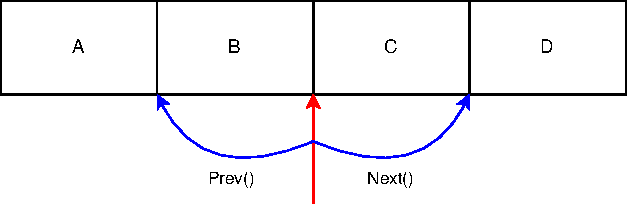
\includegraphics[width=0.5\textwidth]{list_iterator.pdf}
	%\caption{model index}
\end{figure}

下表总结了QListIterator的 API:

%%% Local Variables:
%%% mode: latex
%%% TeX-master: "../../master"
%%% End:

